\documentclass[10pt,a4paper]{report}

\usepackage[utf8]{inputenc}
\usepackage{amsmath}
\usepackage{amsfonts}
\usepackage{amssymb}
\usepackage{graphicx}
\usepackage{color}
\usepackage{enumitem}
\usepackage[top=1cm, bottom=2cm, left=2cm, right=2cm]{geometry}

\usepackage{fancyhdr}
\pagestyle{fancy}

\fancyhead{}
\fancyfoot{} 
\lhead{ \hspace{0.1cm} M1 WI 2014-2015  \hspace{0.4cm} \vline}
\chead{Advanced Algorithms}
\rhead{K.B - K.L - N.R}
\rfoot{\thepage}

\author{Kevin BASCOL, Kevin LAOUSSING, Nicolas REYNAUD}
\title{Algorithmes avancés : \\Problème du voyageur de commerce}

\makeatletter
\renewcommand{\thesection}{\@arabic\c@section}
\makeatother

\begin{document}

\makeatletter
	\begin{titlepage}
	
	\centering
		{
		\vspace*{5cm}
		\hrule height 2pt
		\vspace{0.7cm}
		\Huge \textbf{\@title}}\\
		\vspace{0.7cm}
		\hrule height 2pt
		
		\vfill
		\vspace{1cm}
		\@author\\
		\end{titlepage}
\makeatother
\setcounter{secnumdepth}{4}
\setcounter{tocdepth}{3}
\renewcommand{\contentsname}{Sommaire}
\begingroup\makeatletter
\def\@makeschapterhead#1{%
  {\parindent \z@ \raggedright
    \normalfont
    \interlinepenalty\@M
    \Huge \bfseries  #1\par\nobreak
    \vskip 20pt% <---- à réduire pour avoir plus de place
  }}\makeatother
\tableofcontents
\endgroup
\thispagestyle{empty}
\setcounter{page}{0}
\newpage

\newgeometry{top=2cm, bottom=2cm, left=2cm, right=2cm}

\section{Introduction}
\begin{flushleft}
Le problème du voyageur de commerce, consiste en la recherche d'un trajet minimal permettant à un voyageur de visiter n villes. En règle générale on cherche à minimiser le temps de parcours total ou la distance totale parcourue.\\
Il existe plusieurs approche pour résoudre ce problème, parmi lesquelles on peut distinguer les approches donnant des résultats exactes et les approches donnant des résultats approximatives.
L'objectif de notre projet est d'implémenter ces différentes approches, de pouvoir les tester, de pouvoir analyser les résultats et de déterminer quel est le meilleur compromis entre temps de résolutions et "exactitude" de la solution.
\end{flushleft}


\section{Organisation du projet}

	\subsection{Planning}
	
		\subsubsection{Diagramme de gantt}
		
			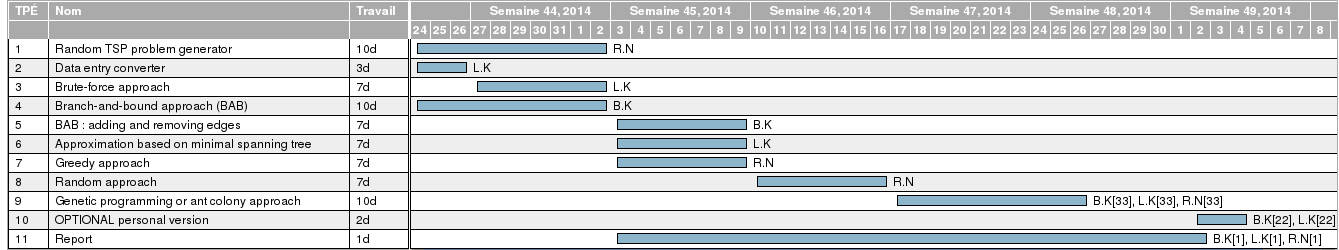
\includegraphics[scale=0.37]{./Ressource/planning_AA.png}
		
	
	\subsection{Langage utilisé et outil de développement}
	\begin{flushleft}
	Nous avons choisi d'implémenter tous nos algorithmes en langage C  pour sa rapidité. En effet les graphes étant garder en mémoire, 
	\end{flushleft}
	
\section{Algorithmes de résolution de problème du voyageur de commerce}

	\subsection{Structure de donnée}
	
	\subsection{Algorithme donnant une solution optimale}
		\subsubsection{Force brute}
		
		\paragraph{Résumé de l'algorithme}
		\begin{flushleft}
		L'algorithme de brute force consiste à explorer toutes les solutions du graphe : c'est-à-dire d'évaluer tous les cycles possibles d'un graphe et de retenir la solution optimale.
		L'avantage est qu'il est simple à implémenter, et qu'il donne la solution optimale.
		Mais son plus grand inconvénient est sa complexité en temps :  $O(n!) \approx O(\exp n)$.
		\end{flushleft}
		\paragraph{Commentaires sur l'implémentation}
		\begin{flushleft}
		L'algorithme a été implémenter en une fonction récursif.
		\end{flushleft}
		\subsubsection{Séparation et évaluation}
		
		\paragraph{Résumé de l'algorithme}
		L'algorithme de séparation et évaluation consiste en un parcours de l'arbre de tous les chemins possible dans le graphe des villes. Mais si le chemin menant à un nœud possède un poids total supérieur à la meilleurs solution trouvée jusque là, alors il ne parcourra pas les sous-arbres de ce nœud.\\
		
		\paragraph{Commentaires sur l'implémentation}
		
		
		
		\subsubsection{Séparation et évaluation avec retrait d'arêtes}		
		
		\paragraph{Résumé de l'algorithme\\}
		L'algorithme de séparation et évaluation avec retrait d'arêtes consiste en un parcours d'arbre. Celui-ci est un arbre binaire, chaque nœud est la matrice des arêtes du graphe, le fils gauche correspond à la matrice résultante du passage par une arête choisie, le fils droit représente la matrice résultante du retrait de cette arête. Le parcours s'arrête au moment où la fonction d'évaluation retourne une valeur supérieur à celle de la meilleure solution trouvée.\\
		
		\paragraph{Commentaires sur l'implémentation\\}
		Je n'ai malheureusement pas réussi à implémenter un programme fonctionnel pour cet algorithme avant la fin du temps imparti. Ceci est en partie dû à la compréhension difficile de l'algorithme, mais aussi à la réalisation chronophage des autres projets universitaires.
		J'ai tenté une version récursive mais me suis embourbé au milieu d'une double récursion.
		
		
	\subsection{Algorithme donnant une solution approximative}
	
		\subsubsection{Approche cupide}
		
		\paragraph{Résumé de l'algorithme\\}
		L'algorithme de l'approche cupide commence par se positionner sur un nœud du graphe. A partir de là, l'algorithme passe au nœud suivant non visité en regardant l'arête avec le poids minimum. Et ainsi de suite jusqu'à avoir parcouru tout les nœuds du graphe.
		
		\paragraph{Commentaires sur l'implémentation\\}
		
		\subsubsection{Approche aléatoire}
		
		\paragraph{Résumé de l'algorithme\\}
		L'approche aléatoire est très simple. L'algorithme se place sur un nœud aléatoire du graphe. A partir de là, l'algorithme passe au nœud suivant non visité en choisissant une arête de manière aléatoire. Jusqu'à revenir à sont point de départ.
		L'algorithme est lancé une première fois. Puis est lancé 100 fois en comparant les résultats entre eux. A chaque fois le chemin avec le coup le moins élevé est choisit.

		\subsubsection{Approche avec l'arbre couvrant de poids minimal}
		\begin{flushleft}
		L'algorithme utilise l'algorithme de Prim ou de Kruskal (dans notre projet, nous avons utilisé l'algorithme de Prim) pour construire un arbre couvrant de poids minimal reliant tout les noeuds du graphe. Une fois que l'arbre couvrant est construite, la solution du problème est donnée par un parcours préfixe de l'arbre.
		L'algorithme est efficace si le distance entre les noeuds respectent la règle de Pythagore. Nous verrons dans le section 4 que cette algorithme donne une solution approximative plus proche de la solution optimale lorsque nous utilisons des graphes du site donnée dans le sujet.
		\end{flushleft}
			
		\paragraph{Commentaires sur l'implémentation}
		
		\begin{flushleft}
		Nous avons utilisé l'algorithme de Prim parce qu'il était plus simple à implémenter. En effet l'algorithme de Kruskal nécessitait d’énumérer toute les arêtes du graphe. Cette opération aurai été trop coûteuse avec la structure de donnée que nous nous sommes donnée.
		\end{flushleft}
		
		\paragraph{Résumé de l'algorithme\\}
		L'algorithme de l'approche génétique passe par plusieurs sous méthode. \\
		Pour commencer une population N de solution est générée. \\
		Cette population est alors modifiée, elle évolue. \\
		l'évolution consiste à trier la population par ordre croissant, à partir de là, un pourcentage d'élite est gardé. Les élites peuvent, avec un faible pourcentage de chance muter. La mutation se traduit par l'inversion de 2 nœuds dans la solution élite. \\
		Le reste de la population subit alors des croisements et des mutations. Les croisement se font sur deux parents. Les parents sont choisit, soit parmi les élites avec un faible pourcentage de chance. Soit parmi une sélection aléatoire de parent parmi les éléments triées. \\
		Le tournois choisit simplement alors la meilleurs solution (Celle avec le cout le plus faible) parmi la sélection aléatoire. \\
		
		Le croisement peut alors commencer. Le croisement comporte alors 2 étapes :
		\begin{itemize}
			\item On commencer par copier une partie de la solution du parent numéro 1. Cette partie est choisit aléatoirement.
			\item On complète ensuite la solution fils obtenu en complétant celle ci par les nœuds présent dans le second parent. En conservant l'ordre présent dans le parent 2.
		\end{itemize}
		Le fils ainsi obtenu à alors un faible chance de muter. \\
		
		L'évolution est ensuite répétée X fois. En prenant comme nouvelle entré la sortie de l'évolution précédente. \\
		Pour finir l'algorithme choisit la meilleurs solution ( Celle avec le plus faible coût ) après évolution . \\
		
		\paragraph{Commentaires sur l'implémentation\\}

\newpage		
\section{Commentaire général sur le code}

Les conventions on été respectée. \\
Qui plus est, nous avons mis un point d'honneur à avoir un code des plus propre possible sur les allocations et libérations de mémoire. \\

Voici le retour de valgrind lancé avec les options : "-v --leak-check=full" sur un graphe à 5 nœuds. \\
\begin{verbatim}
==6610== HEAP SUMMARY:
==6610==     in use at exit: 0 bytes in 0 blocks
==6610==   total heap usage: 29,231 allocs, 29,231 frees, 1,168,096 bytes allocated
==6610== 
==6610== All heap blocks were freed -- no leaks are possible
==6610== 
==6610== ERROR SUMMARY: 0 errors from 0 contexts (suppressed: 0 from 0)
==6610== ERROR SUMMARY: 0 errors from 0 contexts (suppressed: 0 from 0)
\end{verbatim}



\newpage
\section{Etudes d'efficacités des algorithmes}

	\subsection{Graphes générés aléatoirement}
		\subsubsection{Tests temps d'exécution}
			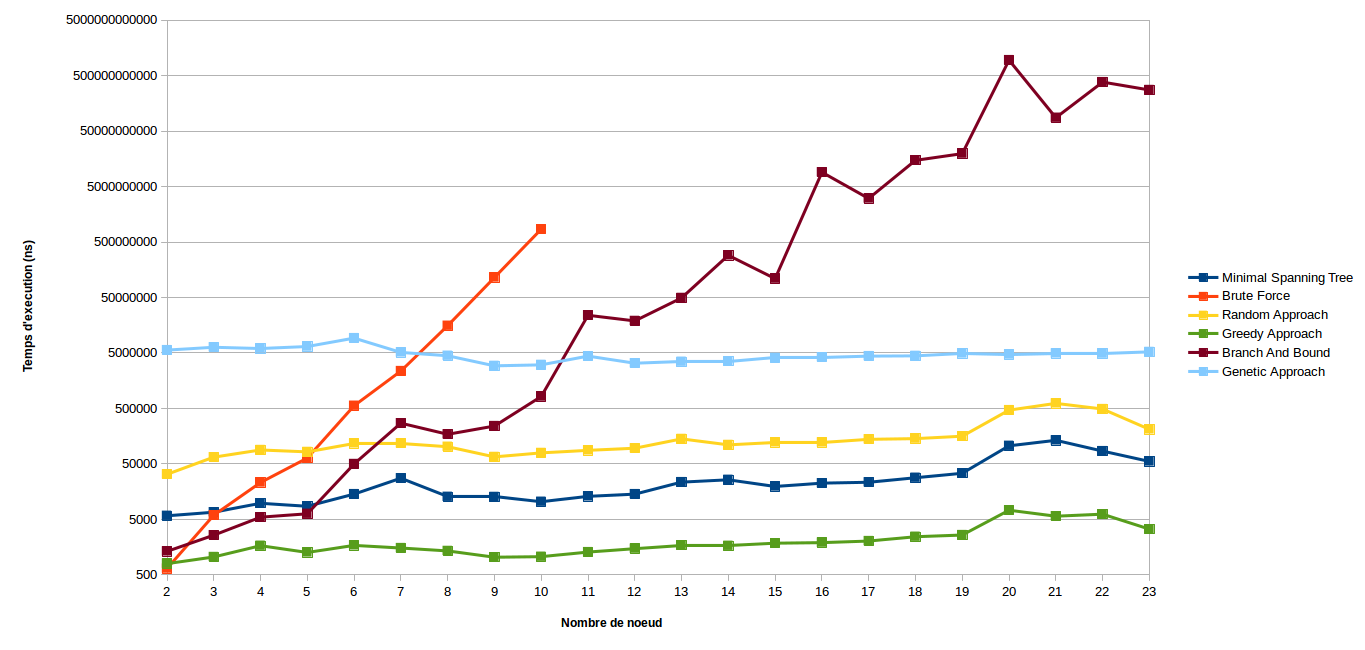
\includegraphics[scale=0.45]{./Ressource/temps_graphes_random.png}
			
			On peut observer qu'à partir de graphes de 8 nœuds, l'algorithme par force brute se termine bien après les autres algorithmes, ce qui est un résultat attendu puisqu'il a la complexité la plus grande.\\
			L'algorithme de séparation et évaluation, quant à lui, devient le plus lent à partir de 11 nœuds. Sa courbe irrégulière est causé par l'élagage qui retire plus ou moins de possibilité selon le graphe.\\
			Les autres algorithmes présentent, à partir de 11 nœuds, une durée plus modérée que les deux précédents et une augmentation de la durée d'exécution plus régulière.
		
		\subsubsection{Tests coût}
			
			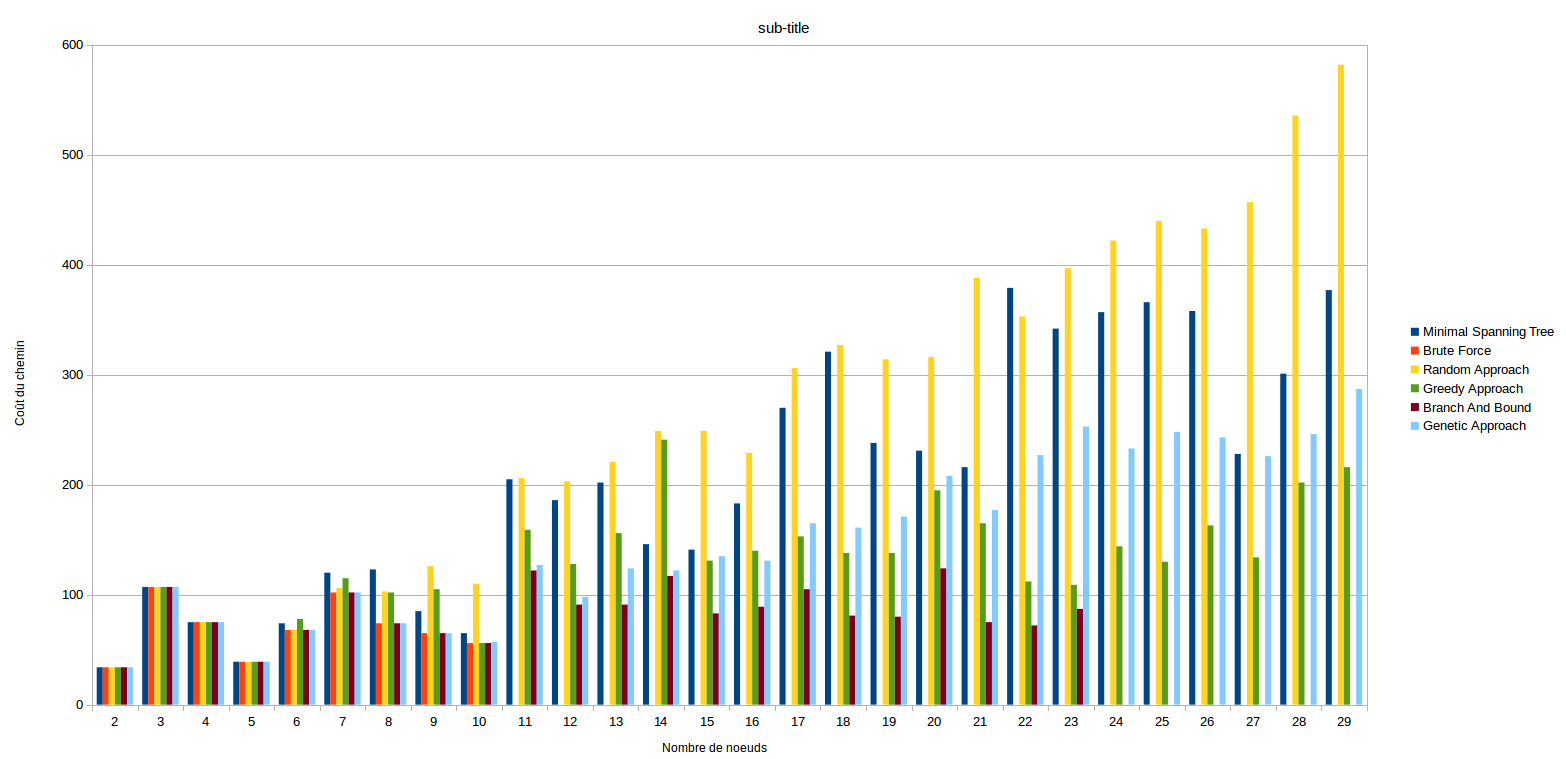
\includegraphics[scale=0.40]{./Ressource/cout_graphes_random.png}
			
			Ici les algorithmes par force brute et de sélection et évaluation donnent toujours une solution avec un poids optimal, ils serviront de repère.\\
			Cet histogramme nous apprend que jusqu'à 7 nœuds tous les algorithmes fournissent une solution quasi-optimale.\\
			A partir de 8 nœuds l'algorithme aléatoire donnera le plus souvent la pire réponse des tests. L'algorithme de l'arbre couvrant donnera la plupart du temps une solution comparable à celle de l'approche aléatoire.\\
			Jusqu'à 21 nœuds, les algorithmes cupide et génétique présentent des résultats comparable mais de plus en plus éloigné de la solution optimale. à partir de 22 nœuds, l'approche cupide est la plus proche de la solution optimale, alors que l'approche génétique s'en éloigne.
					
		\subsubsection{Conclusion}
		Les algorithmes par force brute et de sélection et évaluation sont les seuls donnant toujours une solution optimale. Mais ils présentent aussi le coût en temps extrêmement plus important que les autres, en effet force brute devient inutilisable à environ 10 nœuds et sélection à environ 23 nœuds.
		Parmi les autres algorithmes, l'approche aléatoire est clairement à éviter n'étant pas la plus rapide et étant la moins précise.\\
		L'approche par arbre couvrant est plus rapide que l'approche aléatoire mais est toute aussi imprécise et serait donc à éviter aussi.\\
		L'approche génétique est relativement précise jusqu'à 17 nœuds mais aussi l'une des plus lente et n'est donc pas la meilleure option.\\
		L'approche cupide, quant à elle, est la plus rapide de toutes, mais aussi, la plupart du temps, la plus précise.\\
		
		Donc pour des graphes aléatoires de 2 à 19 nœuds on utiliserait l'algorithme de sélection et évaluation donnant une valeur optimale, et à partir de 20 nœuds on utiliserait l'algorithme cupide.
			
	\subsection{Graphes en ligne}
		\subsubsection{Tests temps d'exécution}
			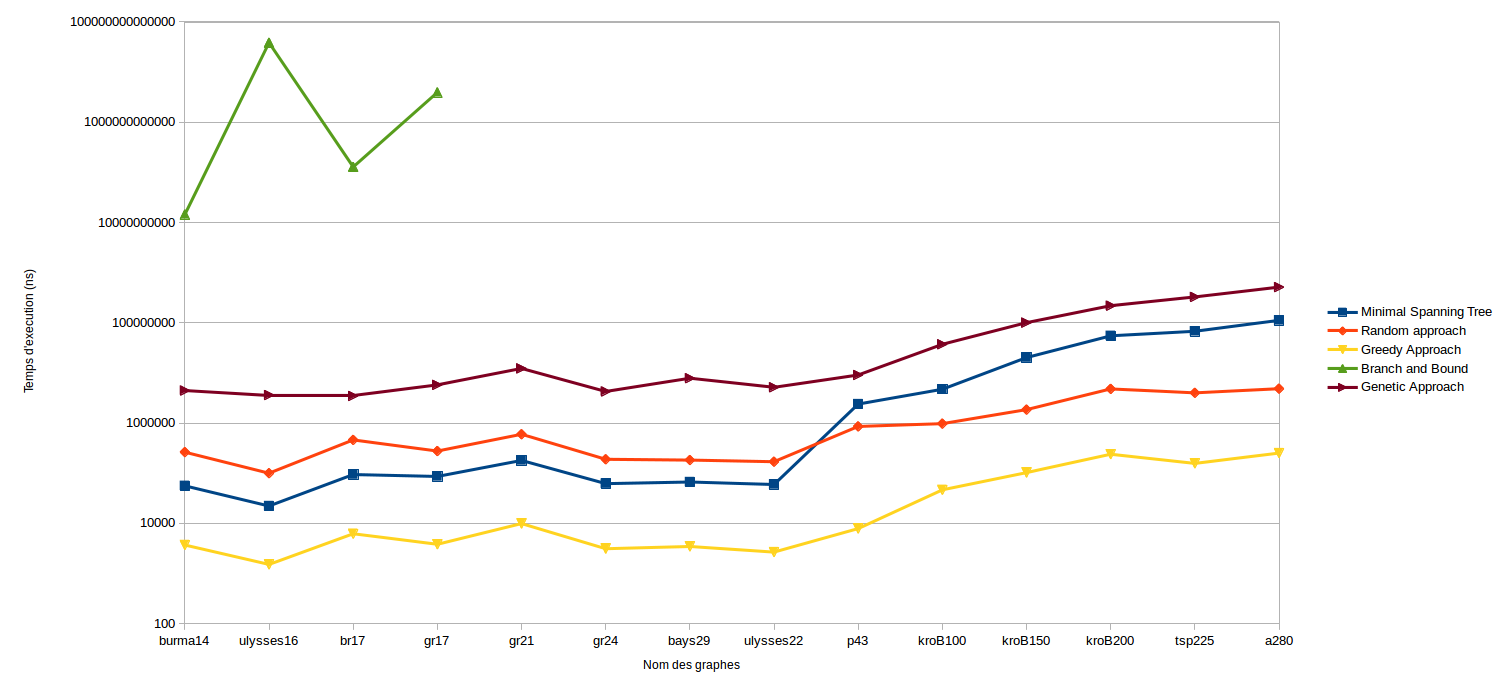
\includegraphics[scale=0.45]{./Ressource/temps_graphes_site.png}
		
	
	\subsubsection{Tests coût}
			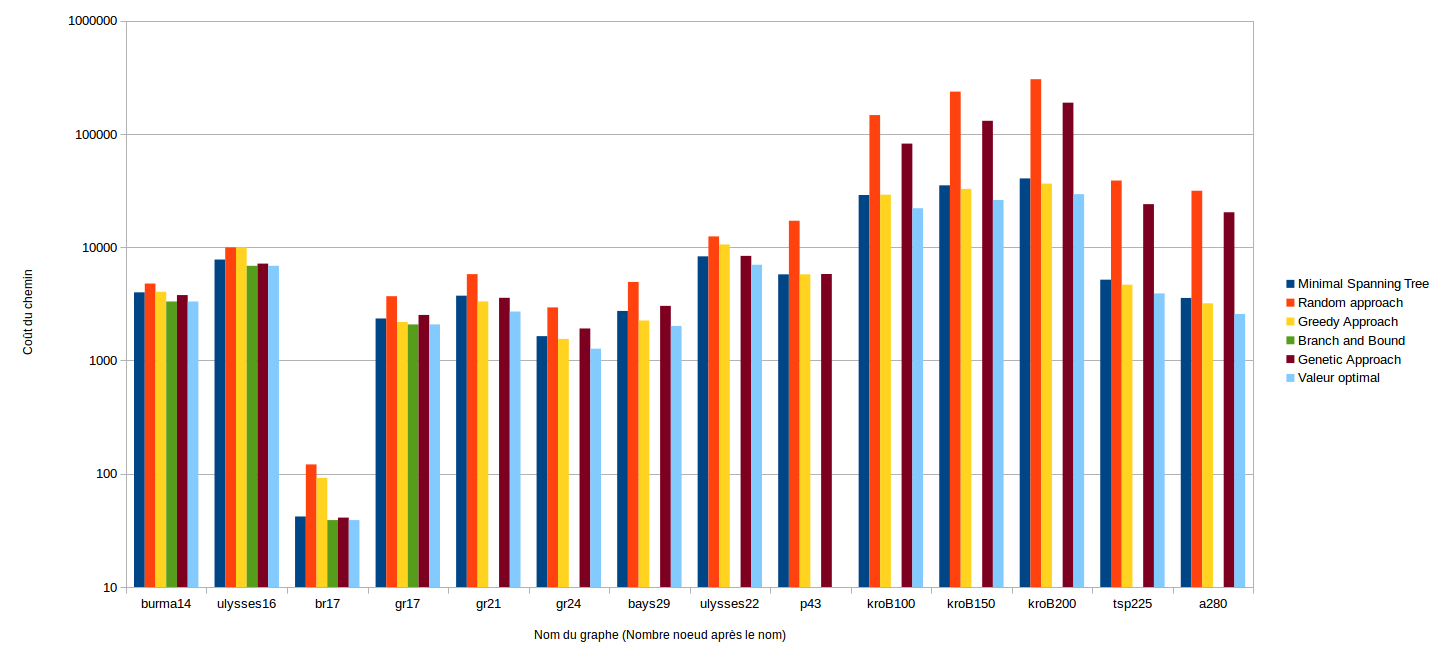
\includegraphics[scale=0.45]{./Ressource/cout_graphes_site.png}
			
	\subsubsection{Conclusion}

\section{Conclusion}
\section{Annexes}

	\subsection{DataConverter}
	
	\subsection{TSPGenerateur}

\end{document}